As mentioned previously, the vertexer used for reconstruction does not accurately propagate track parameters back to the displaced $z$ vertex position. For now, if we assume that by fixing the vertexer we will have resolution good enough to remove the excess high $z$ background events and not lose statistics in the core of the distribution, then we can estimate the reach. Using Equation~\eqref{signal}, the 90$\%$ confidence limit is attained when we can expect 2.303 signal events and greater. Assuming the same number of statistics in the core of the distribution but less background in the high $z$ region, the upper limit reach attainable from the L1L1 data sets is shown in Figure~\ref{fig:L1L1_reach}.

\begin{figure}[htb]
  \centering
      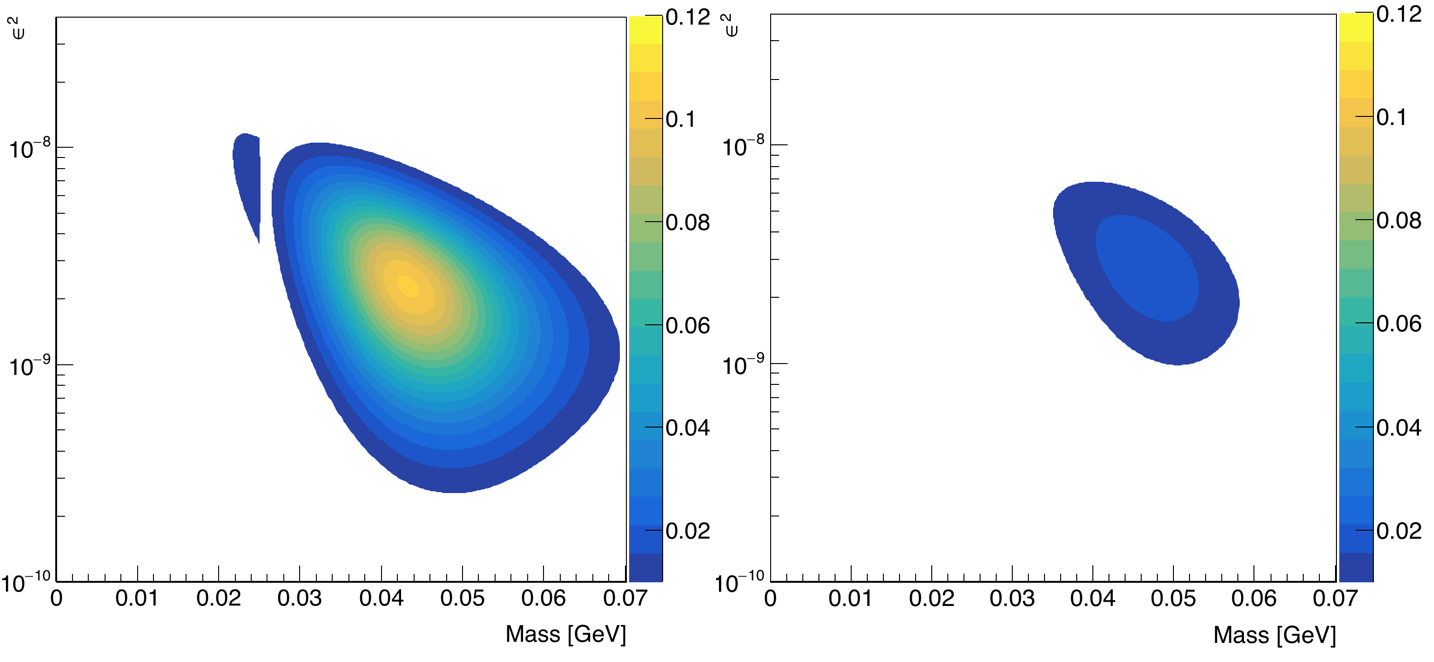
\includegraphics[width=0.9\textwidth]{pics/results/reach_sets.png}
  \caption[Expected signal yield for the individual L1L1 data sets]{The expected signal yield as calculated from Equation~\eqref{signal} is shown for the 0.5~mm L1L1 data on the left and the 1.5~mm L1L1 data on the right. The highest signal expected from the 0.5~mm data is 0.109 events.}
  \label{fig:L1L1_reach}
\end{figure} 

In Figure~\ref{fig:L1L1_reach}, the reach is shown for both the 0.5~mm and 1.5~mm data sets separately. These data sets only contain the reach from the L1L1 components. In the 0.5~mm data, the L1L2 data is contaminated with events in the high $z$ region that push the $zCut$ to be too large to measurable attain any reach. The L1L2 data with the SVT at 1.5~mm has very little contamination of high $z$ background events but has too little statistics to contribute to the reach. Both L2L2 data sets have large backgrounds in the high $z$ region that make fitting a $zCut$ impossible. \\
\indent The combined limits from the 0.5~mm and 1.5~mm L1L1 data sets is shown in Figure~\ref{fig:comb_reach} where the maximum attainable signal is 0.121 events. 

\begin{figure}[htb]
  \centering
      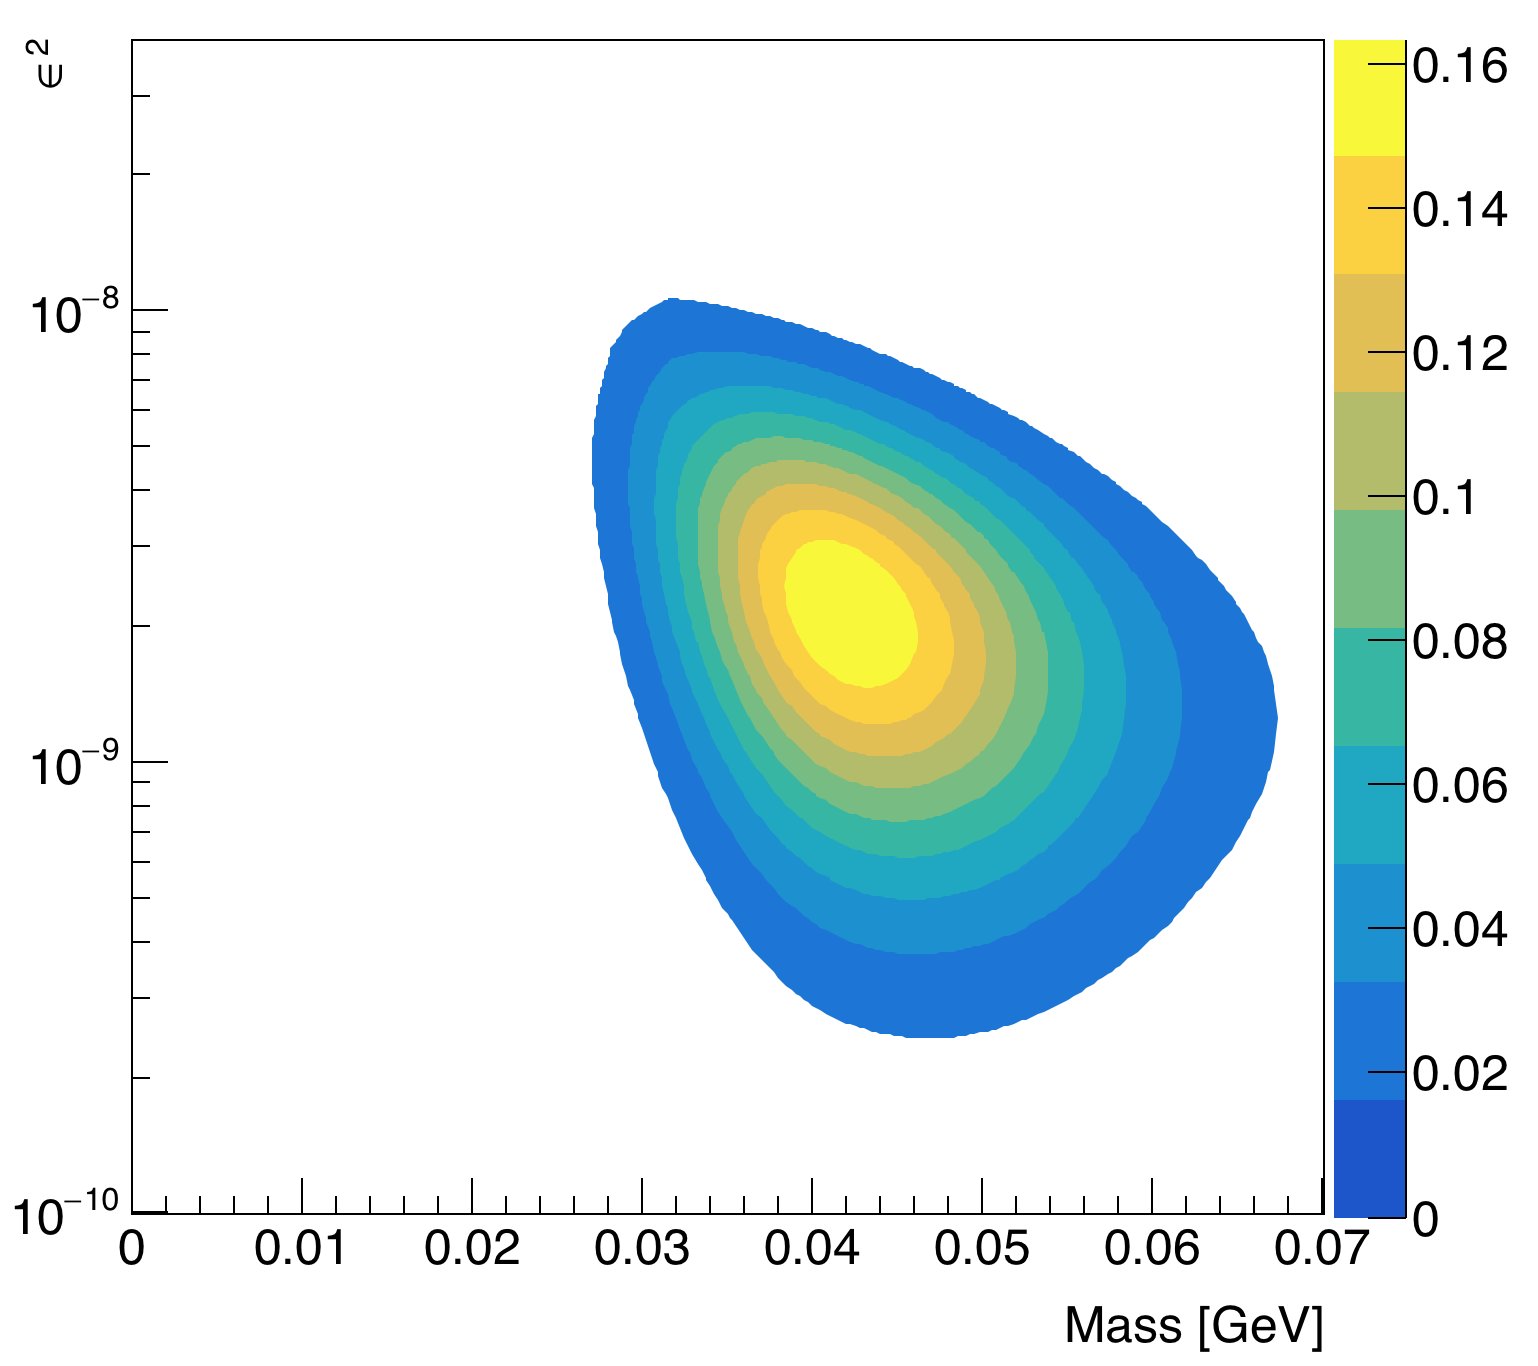
\includegraphics[width=0.55\textwidth]{pics/results/combinedReach.png}
  \caption[Combined reach from all data for the 2015 Engineering Run]{The combined reach for the 0.5~mm and 1.5~mm data is shown with the maximum signal expected to the be 0.121 events.}
  \label{fig:comb_reach}
\end{figure} 

As the maximum signal is significantly less than that required for the 90$\%$ confidence level, no reach was attained for the 2015 Engineering Run. The $zCut$ was projected from the 10$\%$ data to the 100$\%$ data using the following relation obtained from the fits to the vertex distribution (from Equation~\eqref{eq:vtxFit}):
\begin{equation}
\label{eq:zProjected}
z_{2} = z_{1} - l\log(A_1/A_2)
\end{equation}

Here, the subscript 1 indicates the known data where 2 indicates the projected data. The ratio of the amplitudes $A_1/A_2$ of the core distribution is used to estimate the change in statistics, $z$ is the $zCut$, and $l$ is the parameter to describe the length of the exponential tail that varies as a function of mass. By projecting the $zCut$ and the statistics of the 0.5~mm data set, no reach would have been attainable until close to 12~weeks of continuous running. Additionally, the reach that can be obtained for one year of running still covers much less territory in coupling and mass than that expected from the proposal as shown in Figure~\ref{fig:reach_1yr}.

\begin{figure}[htb]
  \centering
      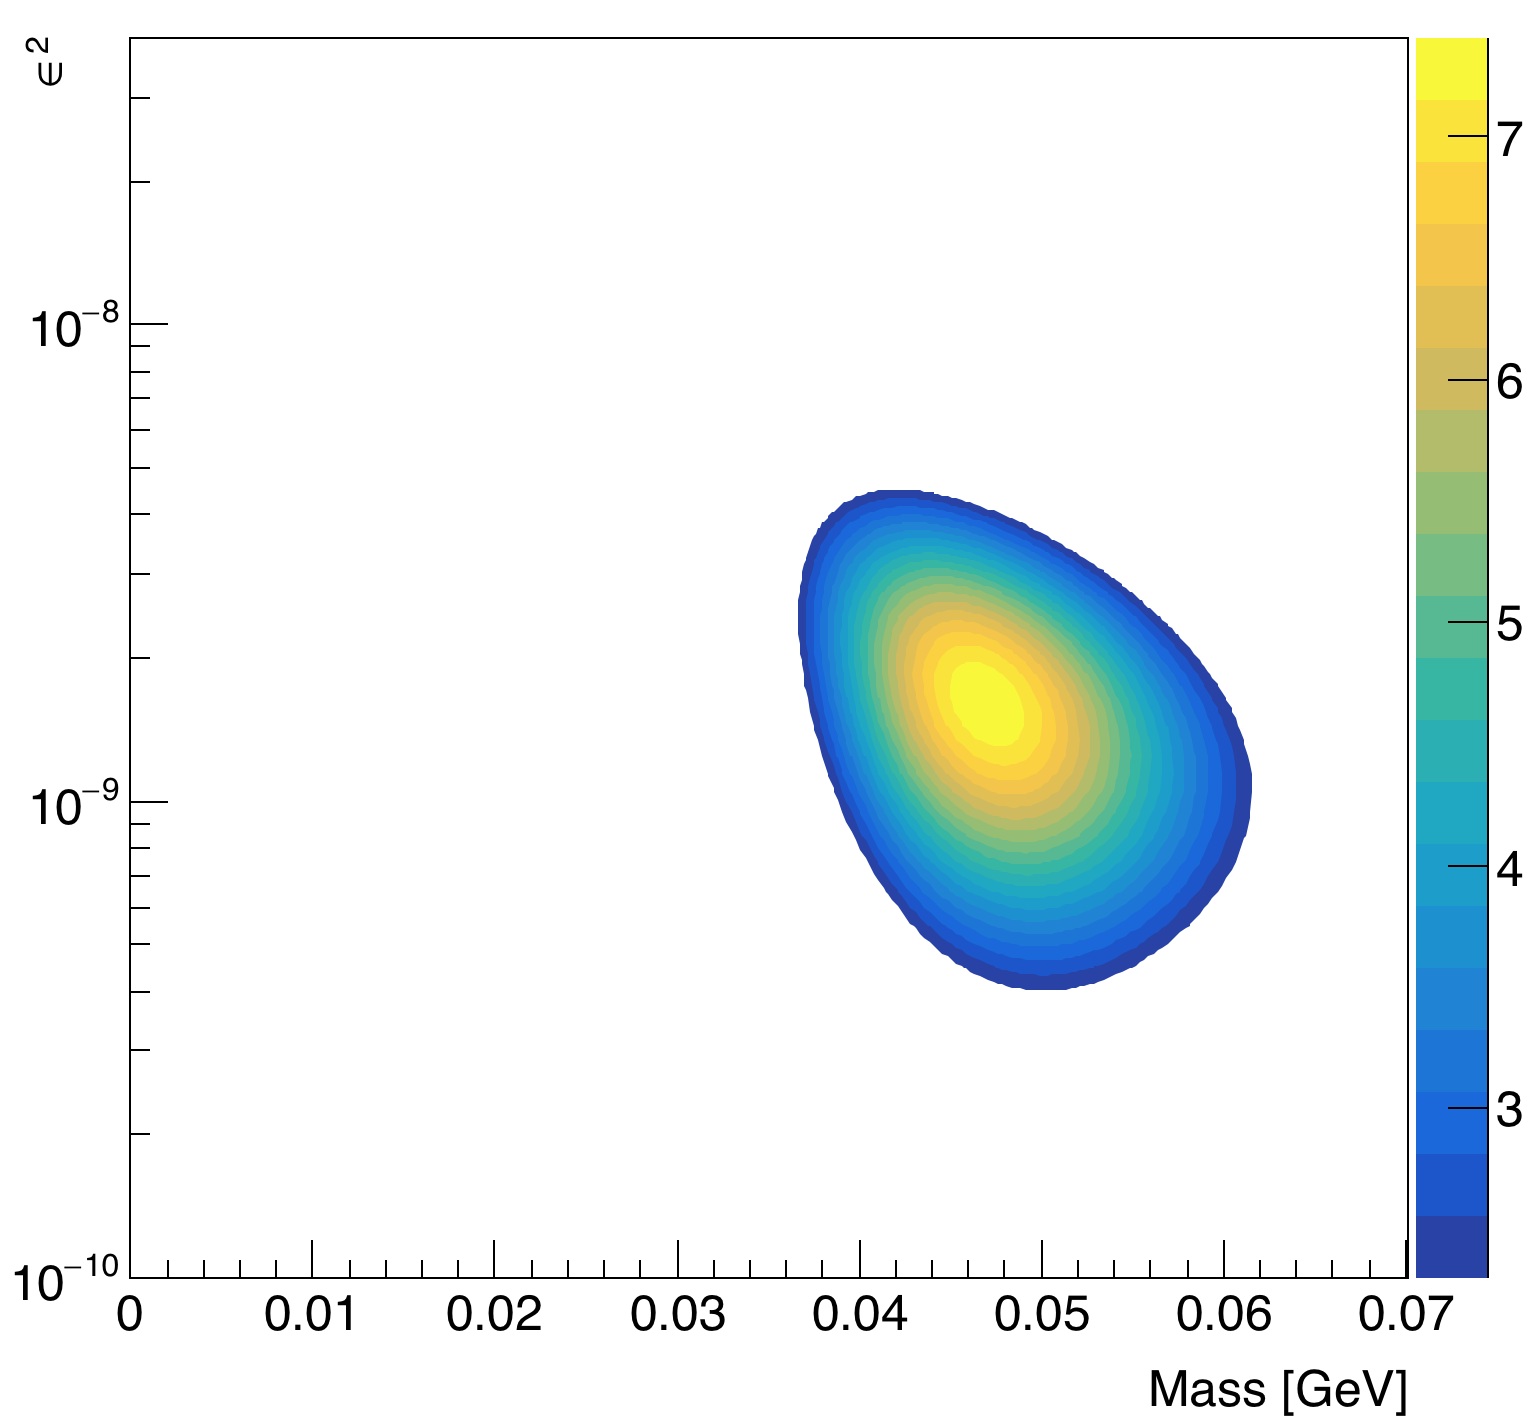
\includegraphics[width=0.55\textwidth]{pics/results/signal_1yr.png}
  \caption[Projected reach for one year of running at 0.5~mm]{By projecting the measured $zCut$ from the L1L1 0.5~mm data and correspondingly increasing the statistics for one year of continuous running, the 90$\%$ CL reach is shown.}
  \label{fig:reach_1yr}
\end{figure} 

While the signal yield is lower, it is interesting to note that for continuous running with the SVT at 1.5~mm, the first reach is attainable at 20~weeks of running. The 90$\%$ CL for 1~year of continuous running is somewhat similar to the the reach projected for the 0.5~mm running but peaks at a slightly higher mass. The background in the 1.5~mm data is much less than the background measured in the 0.5~mm data and is primarily responsible for the improved $zCut$. The 1.5~mm data has a slightly better vertex resolution across the mass range. A comparison of the $z$ vertex resolution is shown in Figure~\ref{fig:vtxRes}. 

\begin{figure}[htb]
  \centering
      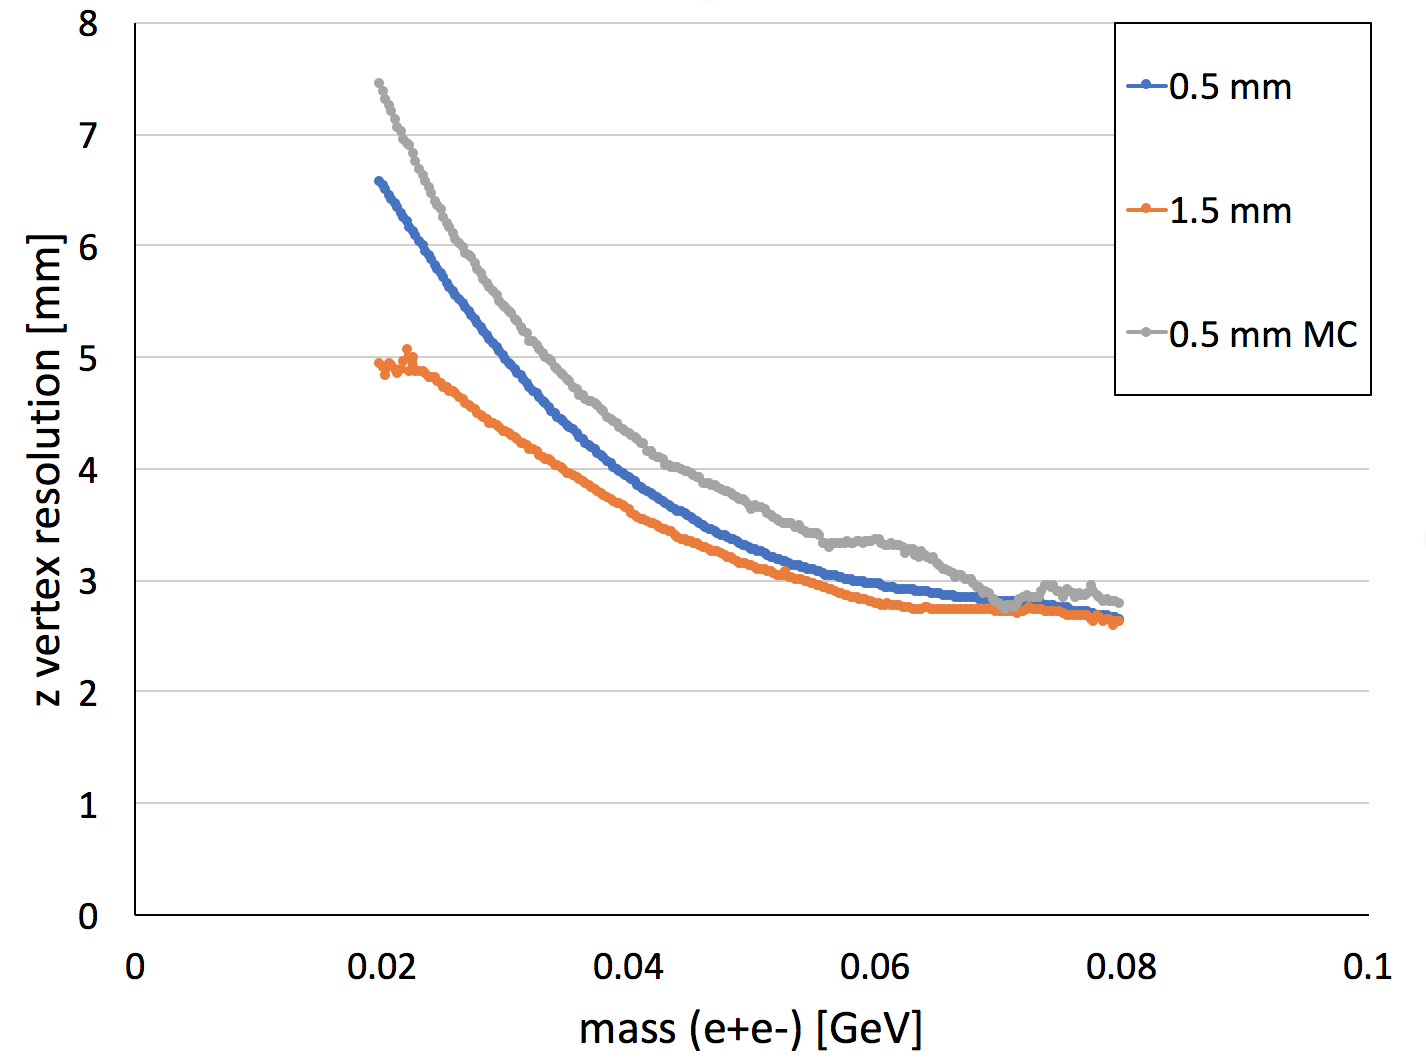
\includegraphics[width=0.75\textwidth]{pics/results/vtxRes.png}
  \caption[Vertex resolutions as measured in data and compared]{The $z$ vertex resolution is shown here as a function of mass where the resolution is obtained from the Gaussian fit to the core of the distribution. The resolution anticipated from MC is slightly worse than what was obtained from the data. The 1.5~mm data has a slightly better vertex resolution than the 0.5~mm data.}
  \label{fig:vtxRes}
\end{figure}

The reach projected from the proposal is very different from that projected from the experimental data. The primary difference between the reach in the proposal and that discussed here is due to the proposal assumption that the reconstructed vertex efficiency was a constant 0.5 between the target and the first layer. This assumption neglected the geometric acceptance effects and loss of smaller masses that decay downstream of the target and miss the first layer. Additionally, this assumption is why the peak in the mass of the proposed reach is much lower (25~MeV as opposed to 42~MeV). The second significant difference is that the hole in the ECal was not accounted for in the reach projections. From data and simulation, we know that we lose trident events when the electron goes through the electron hole, and the event is not triggered. Other differences between the proposal and the measured reach is the thickness of the target (proposed was 0.125$\%$ radiation thickness whereas the measured value was found to be 0.116$\%$), contamination due to excess backgrounds (such as wide angle bremsstrahlung), and time spent running. The wide angle bremsstrahlung triggered many events that were not anticipated and created some downstream $z$ vertex background contamination by interacting with the dead region of Layer 1. \\
\indent Currently, HPS is in the process of developing upgrades that will improve future running. The first upgrade is to add a hodoscope to the positron side of the ECal to prevent triggers from photon clusters from wide angle bremsstrahlung. This improvement in the trigger should reduce some of the background and improve the trident yield. The biggest upgrade to the vertex search is the addition of a Layer 0 SVT tracking plane at 5~cm downstream of the target. Preliminary simulation shows that the vertex resolution is anticipated to improved by a factor of 2 which will enable tighter $zCut$s. This will extend the reach to include efficiency at smaller masses. 